\documentclass[12pt,a4]{article}
\usepackage{graphicx} % Required for inserting images
\usepackage{hyperref}
\usepackage{amsthm,amsmath,amsfonts}
\usepackage{float}
\usepackage{hyperref}
\usepackage[top=1in, bottom=0.5in, right=.75in, left=.75in]{geometry}
\begin{document}
\begin{titlepage}
\begin{center} \includegraphics[width=0.3\textwidth]{tu (1).png}\par
{\large \bfseries Tribhuvan University} \par
{\LARGE \bfseries Institute of Engineering} \par
{\large \bfseries PULCHOWK CAMPUS} \par
{\bfseries Pulchowk, Lalitpur}
~\\~\\
\includegraphics[width=0.10\textwidth]{lines.png}\par
{\bfseries A}\par{\bfseries PROJECT}\par{\bfseries REPORT}\par{\bfseries on}\par
{\Large \bfseries COMPUTER GRAPHICS}~\par
\end{center}
\vfill
\begin{minipage}{8cm}
{\bfseries Submitted By:}\par
Aadarsha Thapa Magar (077BEI002)\par
Manish Kumar Yadav (077BEI022)\par
Mausam Kumar Sah (077BEI23)\par
Pranesh Pyara Shrestha (077BEI030)\par
\end{minipage}
\hfill
\begin{minipage}{7cm}
\begin{center}
{\bfseries Submitted To:}\par
Department of\par Electronics and Computer\par Engineering\par
\end{center}
\end{minipage}
\begin{center}
~\par
    {\bfseries Submitted On:}\par
    March-21,2023
\end{center}
\end{titlepage}
\newpage
\tableofcontents
\newpage
\section{\Huge{Acknowledgement}}
\large{
We would like to express our sincerest gratitude to the campus administration and faculty for their unwavering support and guidance throughout the course of this project. Their knowledge, expertise, and commitment to education have been invaluable in helping me achieve our goals. We would also like to thank our friends for their encouragement and motivation, which has been a constant source of inspiration. Without their support, this project would not have been possible. We are truly fortunate to have had such amazing individuals in our life, and we will always be grateful for their contributions.\\
We express my heartiest indebtedness to our Head of the Department Assoc
Prof. Dr. Jyoti Tandukar for encouragement throughout our project.\\
We also wish to express my deep sense of gratitude to my Project Guide and our Computer Graphics tutor professor Mr.Lok Nath Regmi Department of Computer and Electroics and Communication Engineering  for his  continuous and tireless support and
advice not only during the course of our project but also during the period of our classes.
Finally we express our gratitude to all teaching staff of Department of Computer and Electronics and Communication Engineering  for
their timely support and suggestions.\\
We are conscious of the fact that we have received co-operation in many ways
from the teaching and non-teaching staff of the department of Computer and Electronics and Communication Engineering  and we are grateful to all of their cooperation and their guidance
in completing our task well is time. We thank one and all who have been helped to us
in one way or the other in completing our project on time.

Project Associate\\
Aadarsha Thapa Magar\\ Mausam Kumar Sah\\ Manish Kumar Yadav\\ Pranesh Pyara Shrestha}
\newpage
\section{\Huge{Introduction}}
\large{
As stated the goal of the project was to develop a game highlighting the concepts taught in the
classroom lectures and some knowledge emphasizing the knowledge about the usage of open GL . From the onset the team had high ambitions to develop eye catching
attributes packaged in a game environment.Basically we focuse on building an simple game for controlling the flying object(aeroplane) here in the given path by preventing its collidal from the obstacles that appear with the progression of the game. The initial discussion centered on a dynamic simulation based flying object but gradually shifted to simpler setup where the emphasis would lay on complex graphics
rather than game play mechanics with proper setup of 3d design, lighting models, suitable coloring and many fundamental attributes.
\\
OpenGL graphics library has been used in C
language. The project has been implemented in Microsoft Visual Studio Professional Edition 2008
and 2013 which uses C and/or C++ as the language tool.

OpenGL provide various viewing function that helps us to develop various views of single
object, and the way in which it appears on screen. Orthographic projection is the default view.
OpenGL also provide various transformation functions with the help of these functions user can
render its object at the desired location on the screen. In OpenGL we obtain viewing and modeling
functionality through a small set of transformation functions. We can even rotate the object along
desired locations and with the desired angle on the screen.

OpenGL provides a set of commands to render a three dimensional scene. OpenGL is a
hardware- and system-independent interface. An OpenGL-application will work on every
platform, as long as there is an installed GLUT library.

GLUT is a complete API written by Mark Kilgard which allows us to create windows and
render the 2D or 3D scenes. It exists for several platforms, that means that a program which uses
GLUT can be compiled on many platforms without (or at least with very few) changes in the code.
}
\section{\Huge{Hardware and Software requirements}}
\subsection{\Large{Software Requirements}}
Operating system like Windows XP, Windows 7,Windows 8 and Windows 11 is the platform required to
develop 2D \& 3D graphics applications.
A codeblock C++ compiler is required for compiling the source code to make the executable file which
can then be directly executed.

A built-in graphics library like glut, glut32 \& header file like glut.h and DLL i.e. dynamic link
libraries like glut, glut32 are required for creating the 3D layout.

\subsection{\Large{Hardware requirements}}
The hardware requirements are very minimal and the software can be made to run on most of the
machines.
Processor: Above x86
Processor speed: 500 MHz and above
RAM: 64 MB or above storage space 4GB and more
Monitor Resolution: A color monitor with a minimum resolution of 640*480
2.3 Platform
The package is implemented using Microsoft visual C++ under the windows programming
environment. OpenGL and associated toolkits are used for the package development.\\

\section{\Huge{Methodology}}
\subsection{\Large{Implementation Details}}
\subsubsection{\large{Game Engine}}
The game engine was designed for efficiency, flexibility and extensibility using an object-
oriented approach. Every object in the scene is implemented as a stand-alone object

and it is added to the scene graph at runtime. This has allowed us to implement effects
with great flexibility. For example, shadows and reflections are no more than an
interface that can be applied to any object. Once the interface is implemented, the
engine takes care of actually performing the rendering in the right order to obtain the
desired effect.
\subsubsection{Modelling and Texturing}
{\textbf{\Large{Aeroplane}}\\
The aeroplane() function contains a sequence of OpenGL function calls that translate, rotate, and draw various 3D primitives to construct the airplane model. Here's a brief breakdown of the code:\\

The first four lines of code apply translations and rotations to the airplane model using OpenGL's glTranslated() and glRotated() functions. These transformations change the position and orientation of the airplane in the 3D scene.
The glBegin(GL\_QUADS) call signals the start of a sequence of quad vertices to be drawn using glVertex3f(). Four vertices are provided for each quad, and the vertices are specified in counter-clockwise order as viewed from the front of the quad. The color of the quad is specified using glColor3f().
The code contains several blocks of vertices and colors to draw the various parts of the airplane, including the body, front, rear, and bottom.
Note that the code provided is incomplete and appears to have been truncated. It's missing some vertices and the function ends abruptly without closing the glBegin() block. This would cause a compilation error if used in a complete OpenGL program.\\
\begin{figure}[h]
    \centering
    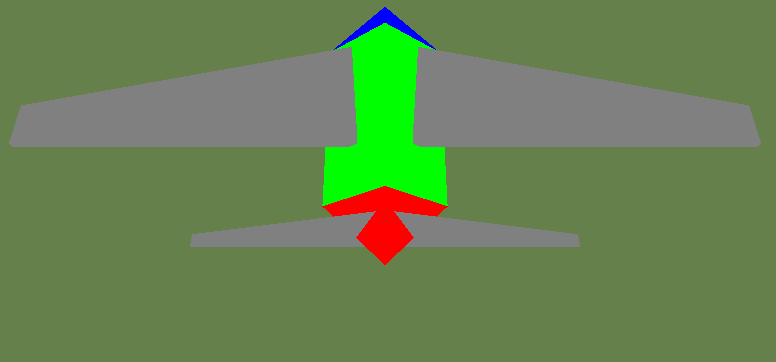
\includegraphics[width=0.8\textwidth]{Screenshot(40).png}
    \caption{Modelling of Aeroplane}
\end{figure}
 \\

 \textbf{\Large{Buildings}}\\
 The function is called "buildings" and takes two integer arguments, "y" and "z".
The first line within the function calls "glPushMatrix()", which saves the current matrix state onto the matrix stack.
The second line uses "glTranslated()" to move the current matrix position to the specified coordinates (-25, y, z).
The third line calls "glutSolidCube()" to draw a solid cube with a size of 45 units.
The fourth line calls "glPopMatrix()" to restore the previous matrix state from the stack.\\
\begin{figure}[h]
    \centering
    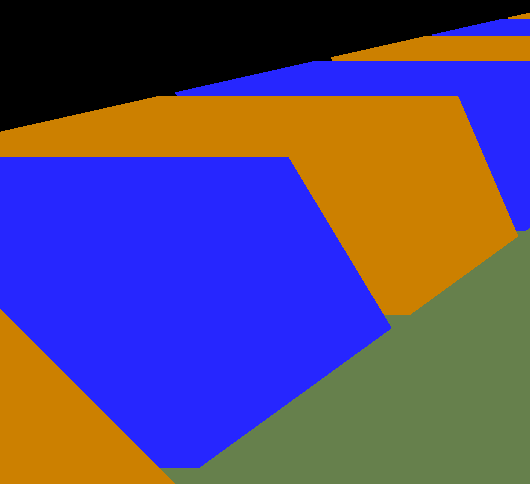
\includegraphics[width=0.4\textwidth,height=4cm]{building.png}
    \caption{Modelling of Building}
\end{figure}
\\ 

\textbf{\Large{Obstacles}}\\
This is a function for drawing a rectangular obstacle in OpenGL. The obstacle is made up of 6 quadrilaterals, each defined by 4 vertices. The first four vertices of each quadrilateral define a rectangle, and the last two vertices define the height of the rectangle.

The function first translates the obstacle by (-15,-5,0) so that it appears at the left of the screen and at a certain height. It then rotates the obstacle by 90 degrees around the y-axis using glRotatef().

Next, it begins drawing the quadrilaterals using glBegin() and ends it with glEnd(). For each quadrilateral, it defines its color using glColor3f(), then specifies its 4 vertices using glVertex3f(). Finally, it repeats this process for each of the 6 quadrilaterals that make up the obstacle.\\
\begin{figure}[h]
    \centering
    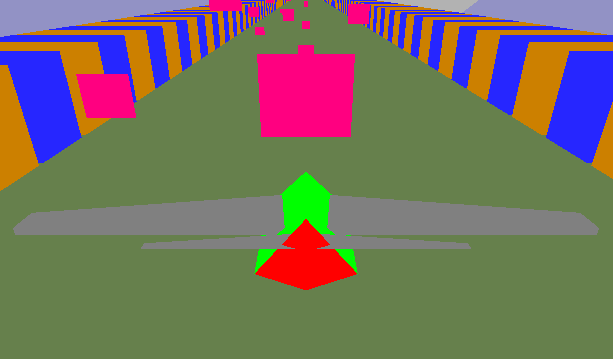
\includegraphics[width=8cm, height=5cm]{Screenshot (58).png}
    \caption{Aeroplane facing different obstacles}
    \label{fig:my_label}
\end{figure}\\
\textbf{\Large{Ground plane and some other obstacles}}\\
It defines a function called Ground that draws a ground plane and places some obstacles on it. The obstacles are drawn using the obstacles() function, which is not shown in the code provided.

The code uses OpenGL functions to perform the drawing, such as glPushMatrix(), glTranslatef(), and glPopMatrix(). These functions are used to save and restore the current state of the matrix stack, as well as to apply translations and rotations to the current matrix.

The function also includes collision detection code that checks if the camera (controlled by the variables angle\_t\_x, angle\_t\_z, and moveground) collides with any of the obstacles. If a collision is detected, the function prints "HIT" to the console
\\
\textbf{\Large{Sun}}\\
It defines a function named "drawsun()" that draws a black circle representing a sun at a particular position in a 3D scene.

The first line of the function "glPushMatrix()" pushes the current matrix onto a stack so that it can be restored later. This is done to avoid any changes made in this function affecting the overall scene.

The next line "glTranslatef(-200,-500,5000);" translates the current position by (-200,-500,5000), which means the circle is moved 200 units to the left, 500 units downwards, and 5000 units away from the camera in the z-axis direction.

The line "glColor3f(0,0,0);" sets the color of the circle to black, as it specifies the RGB values of the color as (0,0,0).

The last line "drawCircle(500,24);" calls another function named "drawCircle" to actually draw the circle with a radius of 500 and divided into 24 segments.

Finally, the function ends with "glPopMatrix();" which restores the previously saved matrix state. This ensures that any subsequent rendering is not affected by the transformations applied in this function.
\begin{figure}[h]
    \centering
    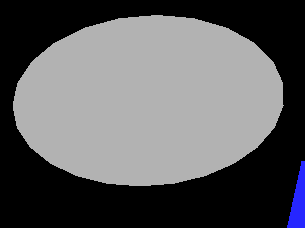
\includegraphics[width=.5\textwidth, height=4cm]{Screenshot (54).png}
    \caption{Sun}
\end{figure}\\

\textbf{\Large{Drawing quadrilateral for various shape}}\\


 It defines a function named "drawEnd()" that draws a quadrilateral shape at a particular position in a 3D scene.

The first line of the function "glPushMatrix()" pushes the current matrix onto a stack so that it can be restored later. This is done to avoid any changes made in this function affecting the overall scene.

The next line "glTranslatef(100,100,0);" translates the current position by (100,100,0), which means the quadrilateral shape is moved 100 units to the right, 100 units upwards, and remains at the same position in the z-axis direction.

The two following lines "glRotated(90,1,0,0);" and "glRotated(90,0,0,1);" apply rotations to the current matrix. The first one rotates around the x-axis by 90 degrees, and the second one rotates around the z-axis by 90 degrees. These rotations can change the orientation of the quadrilateral shape.

The next line "glBegin(GL\_QUADS);" indicates that the following vertices will define a quadrilateral shape.

The four following lines "glVertex3f(0,0,0);" to "glVertex3f(0,0,200);" define the four vertices of the quadrilateral shape, specifying their 3D coordinates in the (x,y,z) format.

The line "glEnd();" ends the definition of the quadrilateral shape.

Finally, the function ends with "glPopMatrix();" which restores the previously saved matrix state. This ensures that any subsequent rendering is not affected by the transformations applied in this function.\\

\subsubsection{Visual Effects}
\textbf{\Large{Display and View}}\\
It defines a function named "display()" that sets up the camera view and displays various 3D objects in a scene.

The first three lines of the function clear the display and set the background color to the values of the global variables red, green, and blue.

$The next several lines set up the camera view. The function gluLookAt() is used to define the camera's position, the direction it is looking in, and its up direction. The parameters are specified as follows: (cameraX, cameraY, cameraZ) for the camera's position, (lookAtX, lookAtY, lookAtZ) for the direction it is looking in, and (upX, upY, upZ) for the camera's up direction. These parameters are controlled by various global variables such as angle\_t\_z, angle\__x, and pos.$

The rest of the function is used to add objects to the scene using various drawing functions such as drawsun(), drawGrid(), Ground(), and aeroplane(). These functions use various OpenGL primitives such as GL\_QUADS, GL\_TRIANGLES, GL\_LINES, and GL\_POINTS to draw 3D shapes.

At the end of the function, the line "glutSwapBuffers();" is used to swap the front and back buffers of the window if double buffering is enabled, which is necessary to display the changes in the scene on the screen.\\

 \textbf{\Large{Animation}}
It defines a function named "animate()" which is responsible for updating the scene during animation. The function has several lines of code that modify the values of various global variables.

The first if statement updates the position of the ground plane by decreasing the value of the variable "moveground" by 0.03 units in the negative Z direction. The ground plane is reset when the value of "moveground" reaches a certain limit.

The next few if statements are used to change the background color of the scene gradually from day to night. They decrease the values of the global variables red, green, and blue until they reach zero.

The variable "angle" is incremented by 0.1 degrees in each frame, which is used to rotate some objects in the scene.

The variable "limit" is also incremented by 0.01 units in each frame and reset to zero when it reaches a certain limit. It is used to control some animations in the scene.

Finally, the function calls "glutPostRedisplay()" to mark the current window as needing to be redisplayed, which is necessary to update the scene in each frame during animation.\\

\begin{figure}[h]
    \centering
    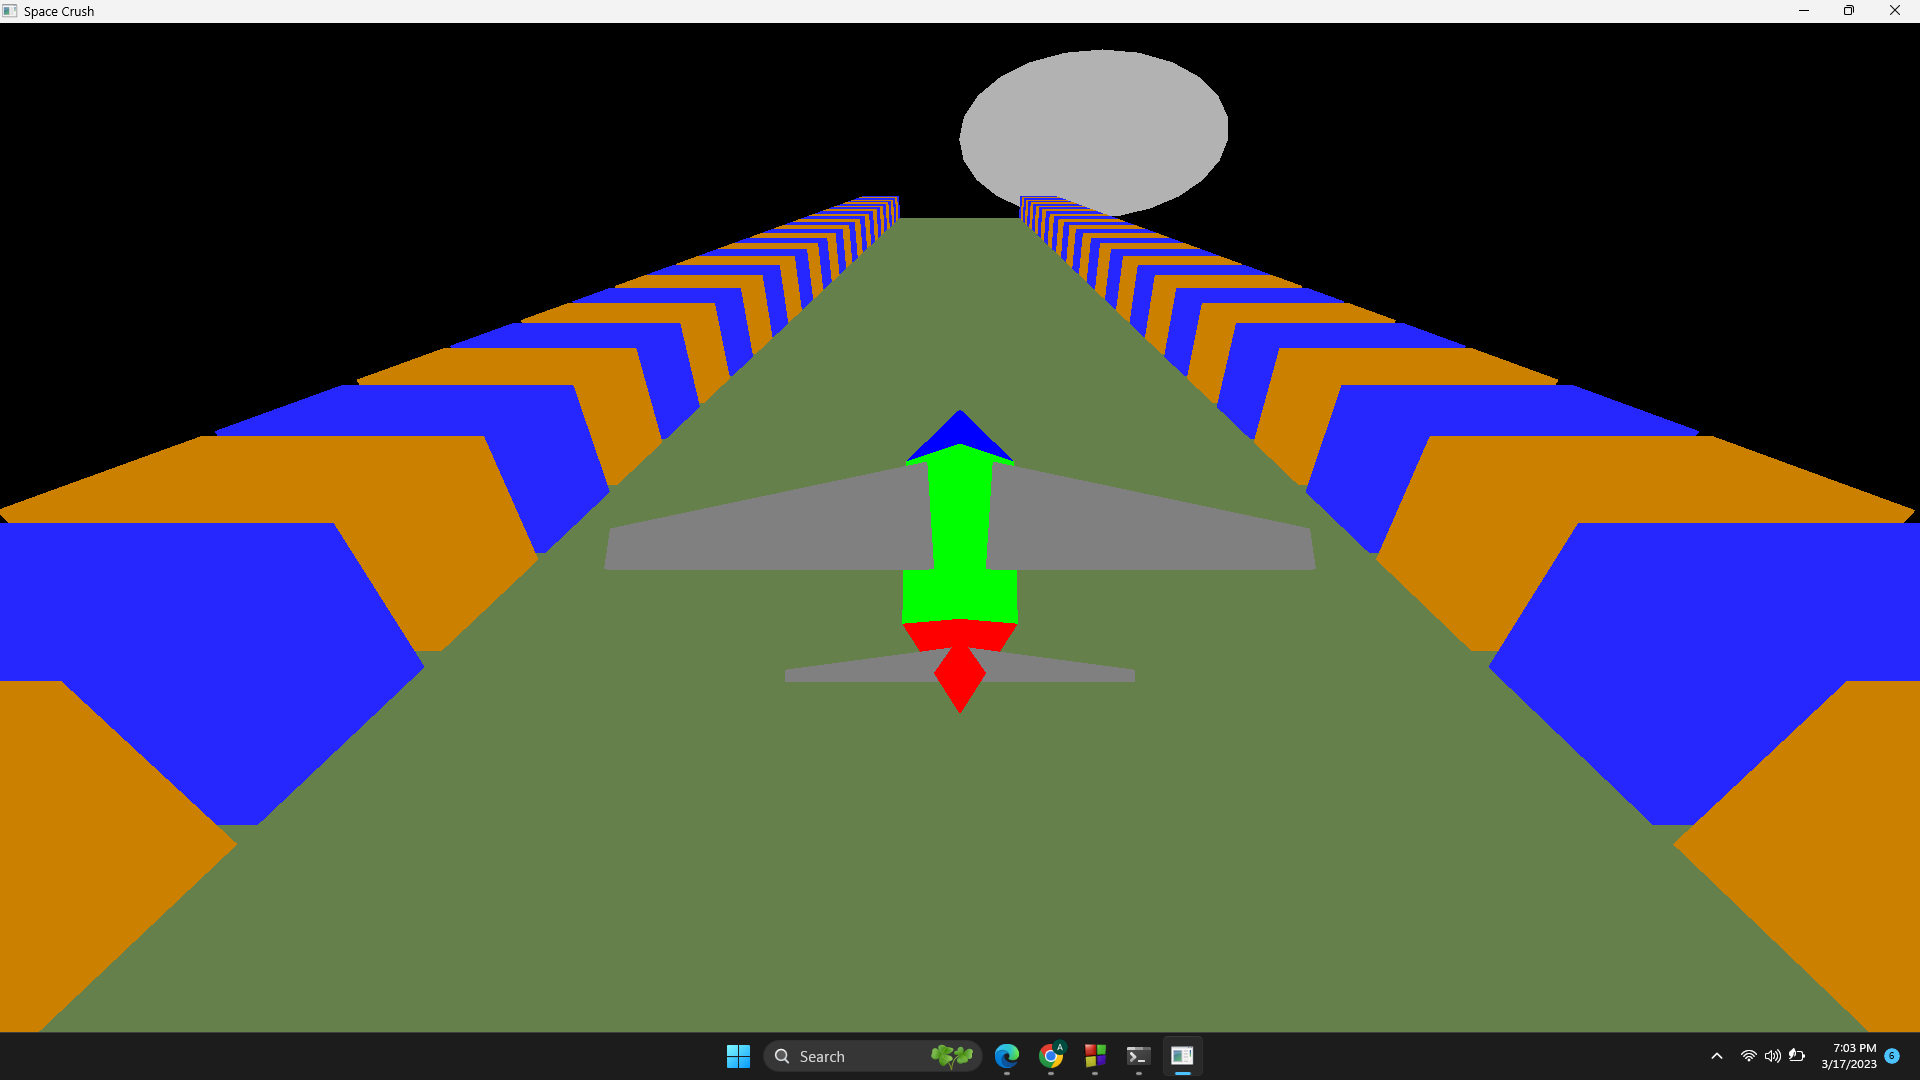
\includegraphics[width=\textwidth, height =14cm]{Screenshot (44).png}
    \caption{A view of gameplay in simulator}
\end{figure}
\subsubsection{Initialization of various variables and components used in Modelling}\\


A function named "init()" which is responsible for initializing the OpenGL graphics environment. The function has several lines of code that set the initial values of various global variables and configure the projection matrix.

The variables "drawgrid" and "drawaxes" are initialized to 0 and 1 respectively, which control whether the grid and axes are displayed in the scene.

The background color is set to black by calling "glClearColor()" with RGB values of 0.

The function then loads the projection matrix by calling "glMatrixMode()" with the argument "GL\_PROJECTION" and initializes the matrix by calling "glLoadIdentity()". The perspective parameters are set using "gluPerspective()" with arguments of 80 degrees for the field of view in the Y direction, an aspect ratio of 1 for the field of view in the X direction, and near and far distances of 1 and 5000.0 units respectively. This sets up a perspective projection with a field of view of 80 degrees and a depth range of 1 to 5000.0 units.

Overall, this function sets up the basic configuration of the OpenGL graphics environment and prepares it for rendering the scene.

The main function takes two arguments: argc (an integer representing the number of command line arguments) and argv (an array of character strings representing the command line arguments).

The program first initializes the position of the camera using the pos variable to set the x, y, and z coordinates. It then initializes three vectors, l, u, and r, which represent the camera's left, up, and right directions, respectively.

Next, the program initializes the game window using the GLUT library by setting its size, position, and display mode.

The program then calls the init function, which initializes various settings for OpenGL, such as the background color.

After enabling depth testing, the program sets up callback functions to handle user inputs such as keyboard and mouse events. The display function is responsible for rendering the graphics, while the animate function is called during idle time to handle animations.

Finally, the program enters the main loop of the OpenGL library using the glutMainLoop function. The program stays in this loop until the user closes the game window.\\
\subsubsection{Implementing the various shape and format}
\textbf{\Large{Axes}}\\
The function name is "drawAxes", and it takes no arguments. Inside the function, there is an if statement that checks whether the global variable "drawaxes" is equal to 1. If it is, then the function proceeds to draw the axes using OpenGL commands.

The axes are drawn as three sets of parallel lines, each set representing one of the three coordinate axes (x, y, and z). The color of each set of lines is set using the glColor3f function, which takes three arguments representing the red, green, and blue color components in the range [0.0, 1.0].

The glBegin(GL\_LINES) and glEnd() functions enclose a set of OpenGL commands that draw a series of line segments between pairs of vertices. In this case, each set of lines is drawn using two calls to glVertex3f, which specify the (x, y, z) coordinates of the starting and ending points of each line segment.

The x-axis is drawn as a green line between the points (-1000,0,0) and (1000,0,0), the y-axis is drawn as a red line between the points (0,-1000,0) and (0,1000,0), and the z-axis is drawn as a blue line between the points (0,0,-1000) and (0,0,1000).

Overall, this function is useful for providing a visual reference for the orientation and scaling of a 3D scene in OpenGL.\\

\textbf{\Large{Grids}}\\
 Function drawGrid() is responsible for drawing a grid of horizontal and vertical lines on the X-Y plane. The grid is centered at the origin and extends to a range of +/- 90 units in both X and Y directions. The grid is drawn using OpenGL's GL\_LINES primitive.

The function takes no arguments and returns nothing. It starts by checking whether the global variable drawgrid is set to 1, which indicates that the grid should be drawn. If drawgrid is not 1, the function exits without doing anything.

If drawgrid is 1, the function sets the drawing color to a light grey using glColor3f(). It then begins drawing the grid using glBegin() and glEnd() functions. Inside the glBegin() and glEnd() block, the function uses a for loop to draw the horizontal and vertical lines of the grid.

For each i value in the range of -8 to 8, the function draws two lines - one parallel to the Y-axis and one parallel to the X-axis. If i is 0, it skips drawing the lines parallel to the main axes to avoid clutter. The coordinates of the lines are calculated using the i value and a constant value of 10, which determines the spacing of the grid lines.
\newpage
\textbf{\Large{Squares}}
There is a function to draw a square with a given size (a) using OpenGL. The square is drawn on the z = 2 plane in the 3D coordinate system.

The function uses glBegin() and glEnd() to define a set of four vertices that form the corners of a quadrilateral. The vertices are specified in counterclockwise order, starting with the top right vertex, and the glColor3f() function can be used to set the color of the square.

Note that glBegin() and glEnd() are deprecated in modern OpenGL and should be avoided. Instead, vertex buffer objects (VBOs) and shaders should be used for improved performance and flexibility.\\

\textbf{\Large{Circle}}\\
There is a  code defines a function draw\_circle\_line that takes in two parameters: radius and segments.

The function generates a set of points on the circumference of a circle using the radius and segments values provided. It then draws lines between these points to create a circle shape. The glBegin(GL\_LINES) and glEnd() functions are used to define the type of primitive to be drawn (in this case, lines) and to indicate the end of the set of vertices to be drawn.

The circle is drawn using the glVertex3f function, which takes in the x, y, and z coordinates of a point. In this case, the z coordinate is set to 0, as the circle is being drawn in a 2D plane.\\


\textbf{\Large{Cylinder}}\\
 A function draw\_cylinder which takes three arguments: radius (the radius of the cylinder), height (the height of the cylinder) and segments (the number of segments used to approximate the cylinder).

The function first initializes a two-dimensional array points of size 2 by 100 to store the x, y, and z coordinates of the vertices that make up the cylinder. The for loop generates the x and y coordinates for the bottom and top of the cylinder, and sets the z coordinates to 0 for the bottom and height for the top.

The for loop then creates a series of quadrilaterals to form the sides of the cylinder using glBegin(GL\_QUADS) and glEnd() OpenGL functions. The colors of the quadrilaterals alternate between different shades of purple based on the i value.

Overall, this function generates a cylinder using OpenGL primitives and can be used in a larger graphics program to display 3D objects.\\

\newpage
\textbf{\Large{Cone}}\\
A function draws a cone with a circular base, given the radius, height, and number of segments. It uses a loop to generate points on the base of the cone, and then another loop to draw triangles between these points and the tip of the cone.

The shading effect is created by interpolating between two colors (purple and black) based on the position of each triangle in the loop. The shade variable is calculated using a simple linear function that maps the position of the triangle to a value between 0 and 1, and then the red and blue color components are set to this value, while the green component is always 0.

Note that there is a hardcoded limit variable that determines how many triangles are drawn, which is subtracted from the total number of segments. This is probably to prevent the apex of the cone from being too pointy, but it would be better to use a more flexible method that adjusts the limit based on the radius and height of the cone.

Overall, this is a simple and effective implementation of a cone using OpenGL primitives.\\

\textbf{\Large{Sphere}}\\
a function named drawSphere that takes in three parameters: radius, slices, and stacks. It is written using the OpenGL graphics library and generates a sphere made up of quads using the specified radius, slices, and stacks parameters.

The function begins by defining a 2D array of point structures, where each structure contains an x, y, and z coordinate. The number of elements in each dimension of this array is determined by the stacks and slices parameters, respectively.

Next, the function uses nested for loops to iterate over each point in the array and calculate its x, y, and z coordinates using the radius, slices, and stacks parameters. The resulting array of points is used to draw the sphere using OpenGL's GL\_QUADS primitive.

The function iterates over the array of points and for each pair of adjacent points, it defines a quad using glBegin(GL\_QUADS) and glEnd() function calls. The color of each quad is defined using glColor3f().

The quads are generated using the following vertices:\\

The current point\\
The point to the right of the current point\\
The point directly below the current point and to the right\\
The point directly below the current point\\
This generates a series of horizontal rings that are then connected by vertical quads to form the spherical shape. The second hemisphere is drawn similarly by negating the z coordinate of each point.\\

\textbf{\Large{3D rectangle and quadrilateral}}\\
There is a function called "quad" that draws a 3D rectangle or quad using OpenGL. It uses the glBegin() and glEnd() functions to define the start and end of a set of vertices that form a polygon.

Inside the glBegin() and glEnd() block, there are multiple calls to glVertex3f() that define the vertices of the quad. Each call specifies the x, y, and z coordinates of a vertex.

The quad is made up of six faces, each with a different color specified using glColor3f(). The order in which the vertices are specified determines the orientation of each face, and thus the direction in which it is visible.

Note that glBegin() and glEnd() are deprecated in modern versions of OpenGL and should not be used in new code. Instead, vertex buffer objects (VBOs) and shaders are typically used for rendering 3D graphics.\\

\textbf{\Large{Scene of objects used}}\\
 A function called drawSS which appears to be used to draw a simple scene consisting of three spheres, each of which is rotated and translated relative to the others.

The function begins by calling another function called draw\_circle\_line which is not shown here, so it is unclear what this function does exactly.

Next, the code sets the current drawing color to red using glColor3f, and then calls a function called drawSphere to draw a large sphere with a radius of 20 and a resolution of 30 by 30. The next few lines of code apply a series of translations and rotations to the current coordinate system using glRotatef and glTranslatef, and then draw two smaller spheres in green and blue respectively, using drawSphere with radii of 15 and 10. The blue sphere is enclosed in a glPushMatrix/glPopMatrix block, which means that the transformations applied to the coordinate system within this block do not affect the transformations outside the block.

Finally, the code sets the drawing color back to white using glColor3f, and there is some commented-out code at the end which appears to be an attempt to draw a square, but it is currently disabled.
\newpage
\subsubsection{Rendering and 3D movement}
he code first calls a function called draw\_circle\_line with parameters 110 and 40, which I assume is a function that draws a circle. Then it sets the color to red with glColor3f(1,0,0) and calls the drawSphere function with radius 20 and 30 slices and stacks. This should draw a red sphere.

Next, the code calls glPushMatrix to save the current transformation state, then applies some transformations to the current matrix. It rotates by the angle variable around the z-axis with glRotatef(angle,0,0,1), then translates by 110 units along the x-axis with glTranslatef(110,0,0), and finally rotates again by 2 times the angle around the z-axis with glRotatef(2*angle,0,0,1). After these transformations, the color is set to green with glColor3f(0,1,0) and another sphere is drawn with radius 15 and 30 slices and stacks. This sphere will be smaller and appear to orbit around the center of the first sphere due to the applied transformations.

Finally, the code calls glPopMatrix to restore the previous transformation state, then pushes the matrix again and applies another set of transformations. It sets the color to magenta with glColor3f(1,0,1) and rotates by the angle variable around the y-axis with glRotatef(angle,0,1,0). Then it translates by 110 units along the x-axis with glTranslatef(110,0,0) and rotates by 2 times the angle around the z-axis with glRotatef(2*angle,0,0,1). Another green sphere is drawn with radius 15 and 30 slices and stacks, which will appear to orbit around the first green sphere.

Overall, it looks like the code is creating an animation of two spheres orbiting around a larger sphere. The angle variable is likely being incremented over time to make the spheres move.\\
\begin{figure}[h]
    \centering
    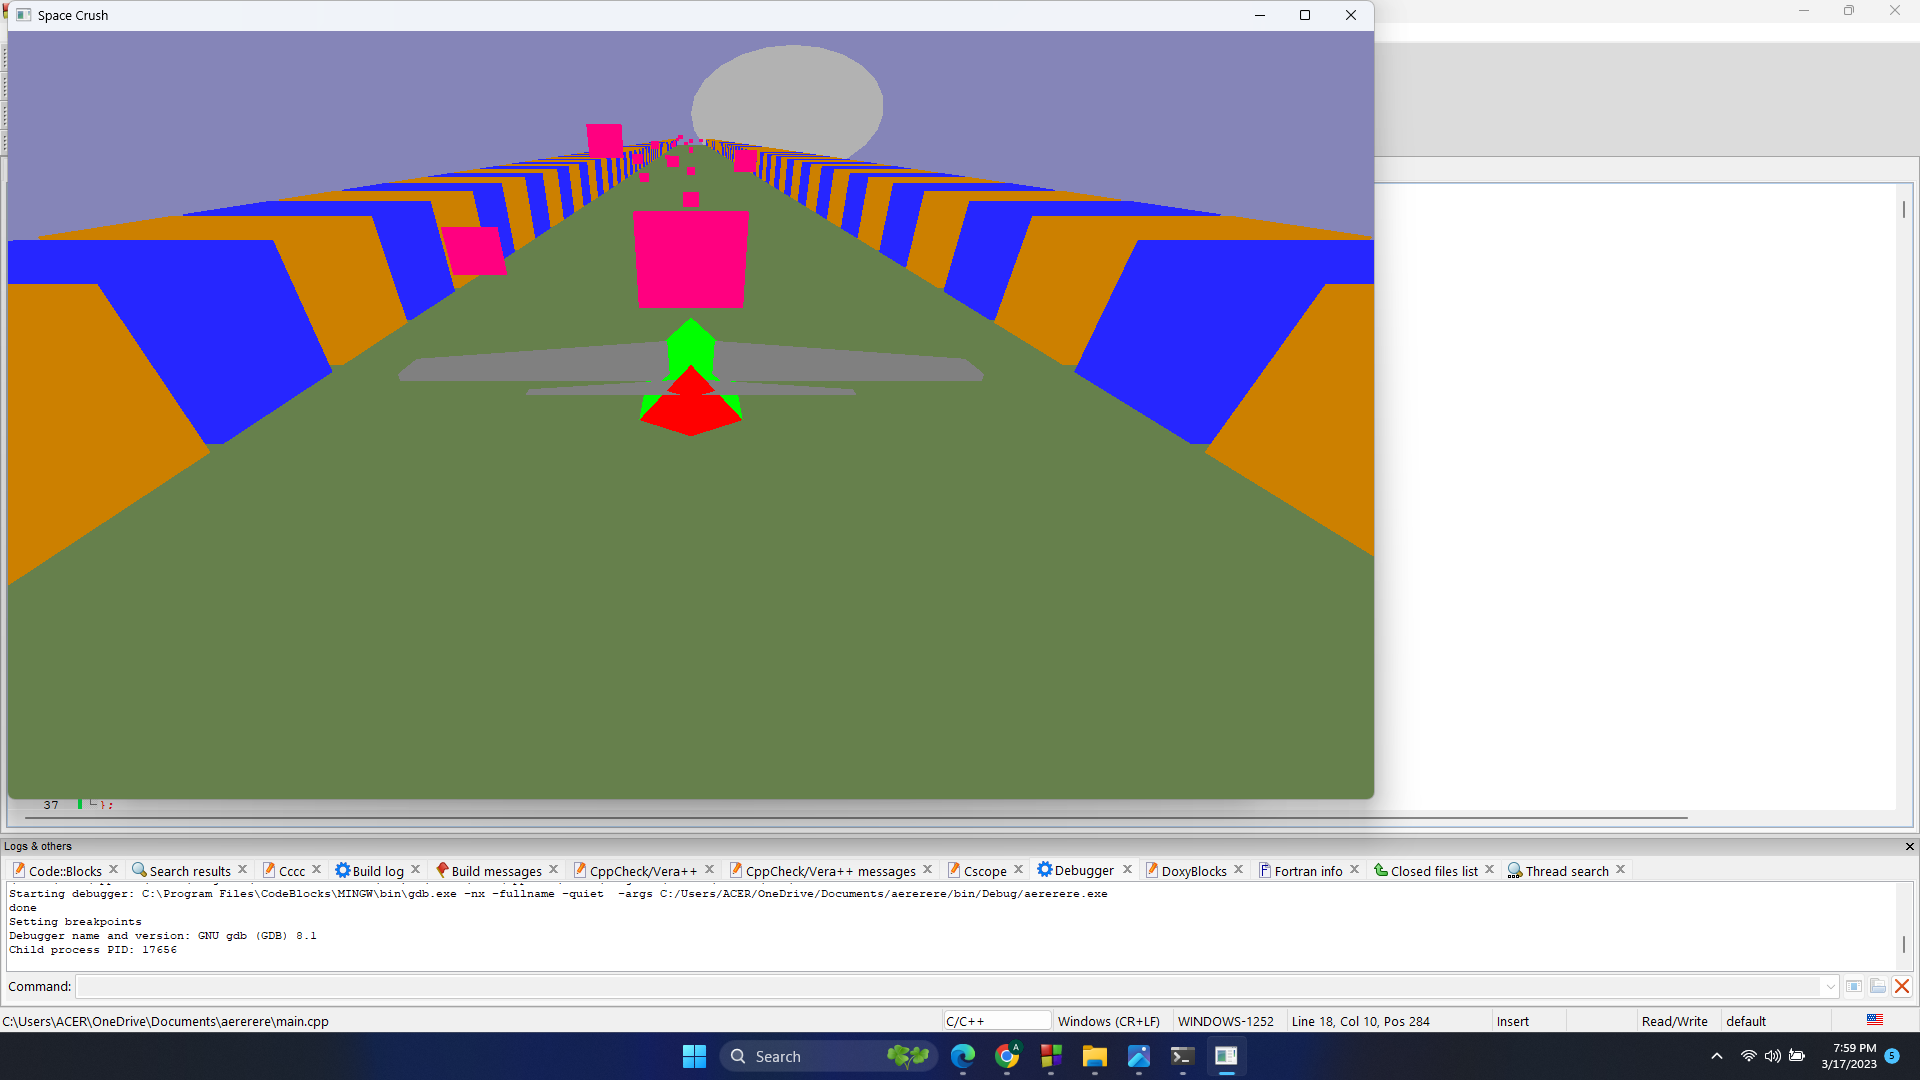
\includegraphics[width=0.8\textwidth,height=7cm]{Screenshot (59).png}
\end{figure}\\
\newpage
\subsubsection{Control of gameplay }
\textbf{\Large{Control through keyboard}}\\
There appears to be a keyboard listener function in OpenGL using C++. When a key is pressed, the function checks which key was pressed and performs a certain action depending on the key.

If the key 'w', 's', 'a', or 'd' is pressed, the function calls the "resetpos()" function. This function is likely responsible for resetting the position of the object being rendered by the OpenGL program.

If any other key is pressed, the function checks the values of "angle_c_x" and "angle_c_z" and adjusts them based on their current values. It appears that these variables are used to control the rotation of an object in the OpenGL program.

\\

There is a function written in C++ that serves as a keyboard listener for a graphics program. It takes three parameters: an unsigned character "key", and two integers "xx" and "yy". The function performs different operations depending on the key pressed, such as rotating the camera and adjusting angles.

The function first initializes three double variables "x", "y", and "z", and a double variable "rate". The rate variable is set to 0.01, which is used to control the amount of rotation applied.

The function then uses a switch statement to perform different actions depending on the key pressed. For example, if the key pressed is '1', the function rotates the camera and updates its position. If the key pressed is 'w', the function adjusts the camera's angle of rotation around the z-axis.

The function uses trigonometric functions such as "cos()" and "sin()" to calculate the new camera position and orientation after rotation.

Finally, the function updates various global variables such as "angle\_c\_x" and "angle\_c\_z", which are used to keep track of the camera's current angles of rotation.\\
\begin{figure}[h]
    \centering
    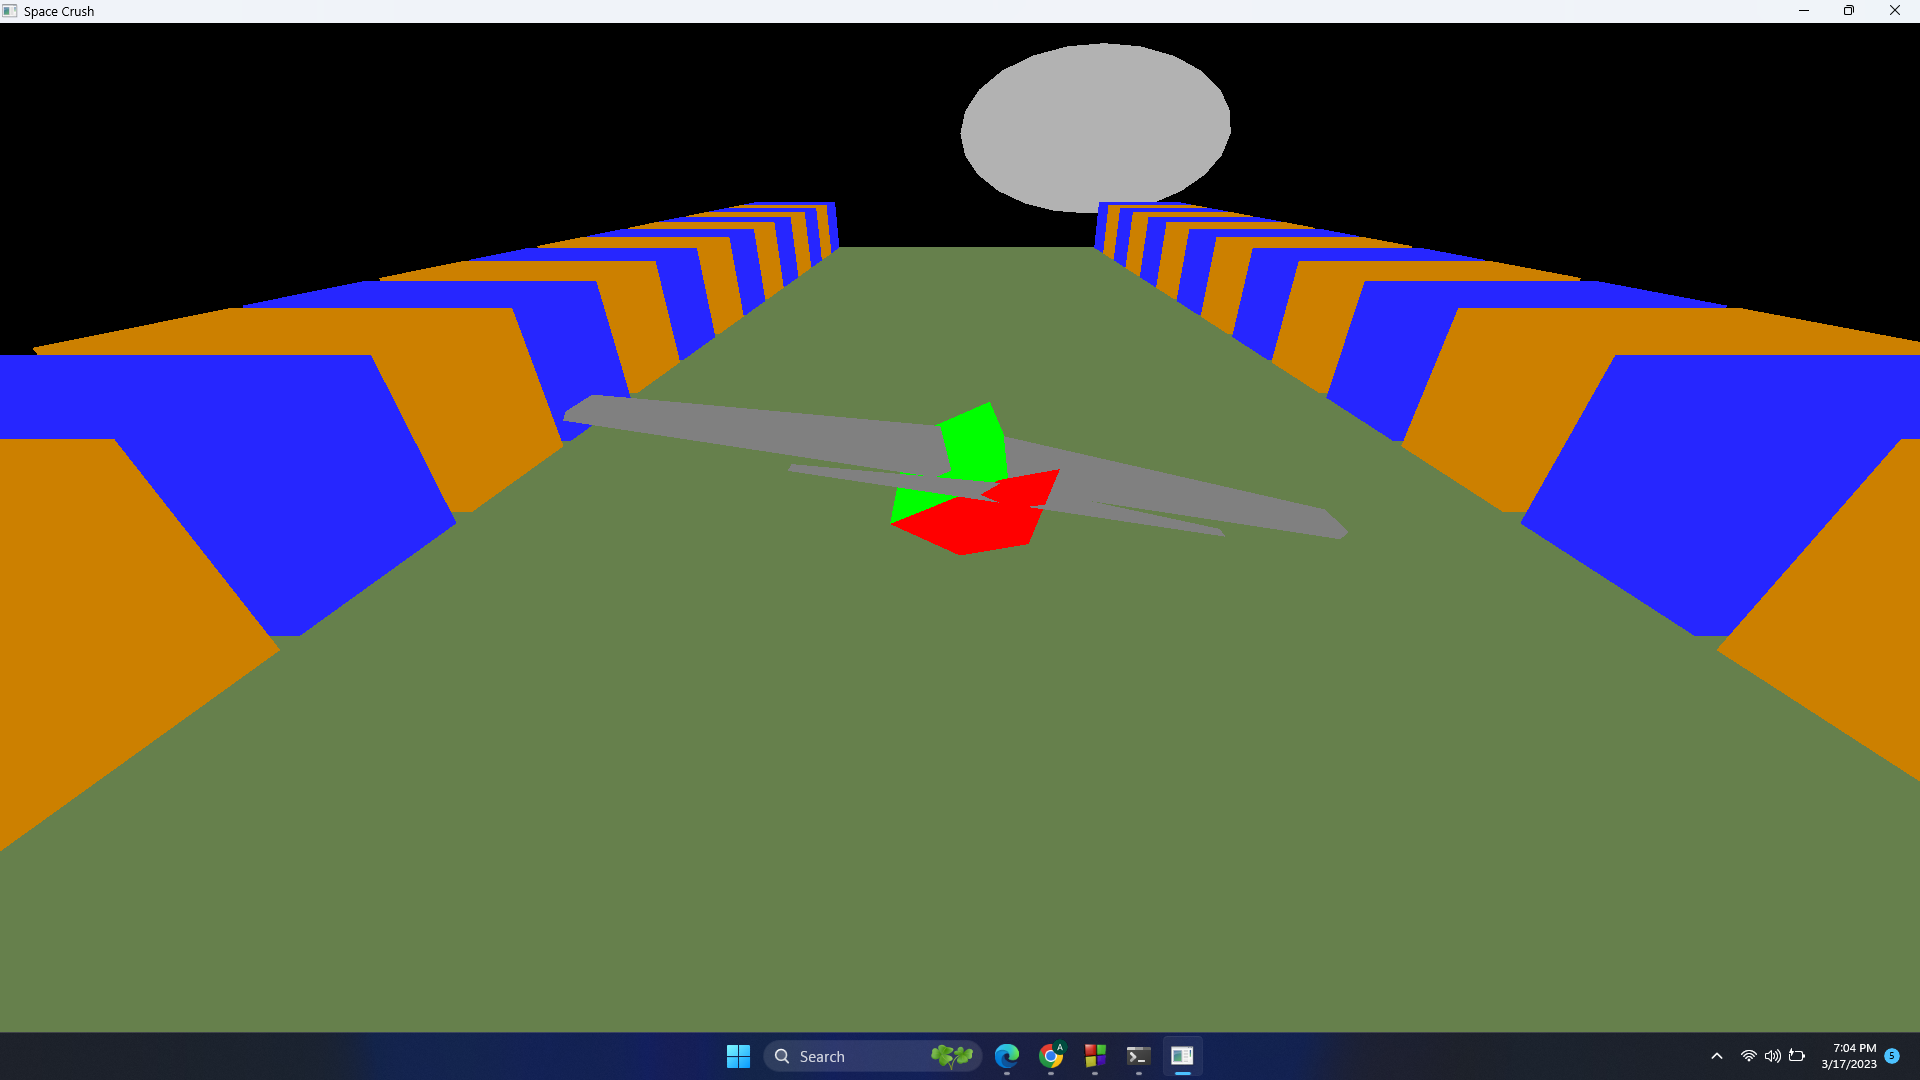
\includegraphics[width=0.7\textwidth, height=5cm]{Screenshot (51).png}
    \caption{Right tilt by pressing 'D' key}
    \label{fig:my_label}
\end{figure}\\

\begin{figure}[h]
    \centering
    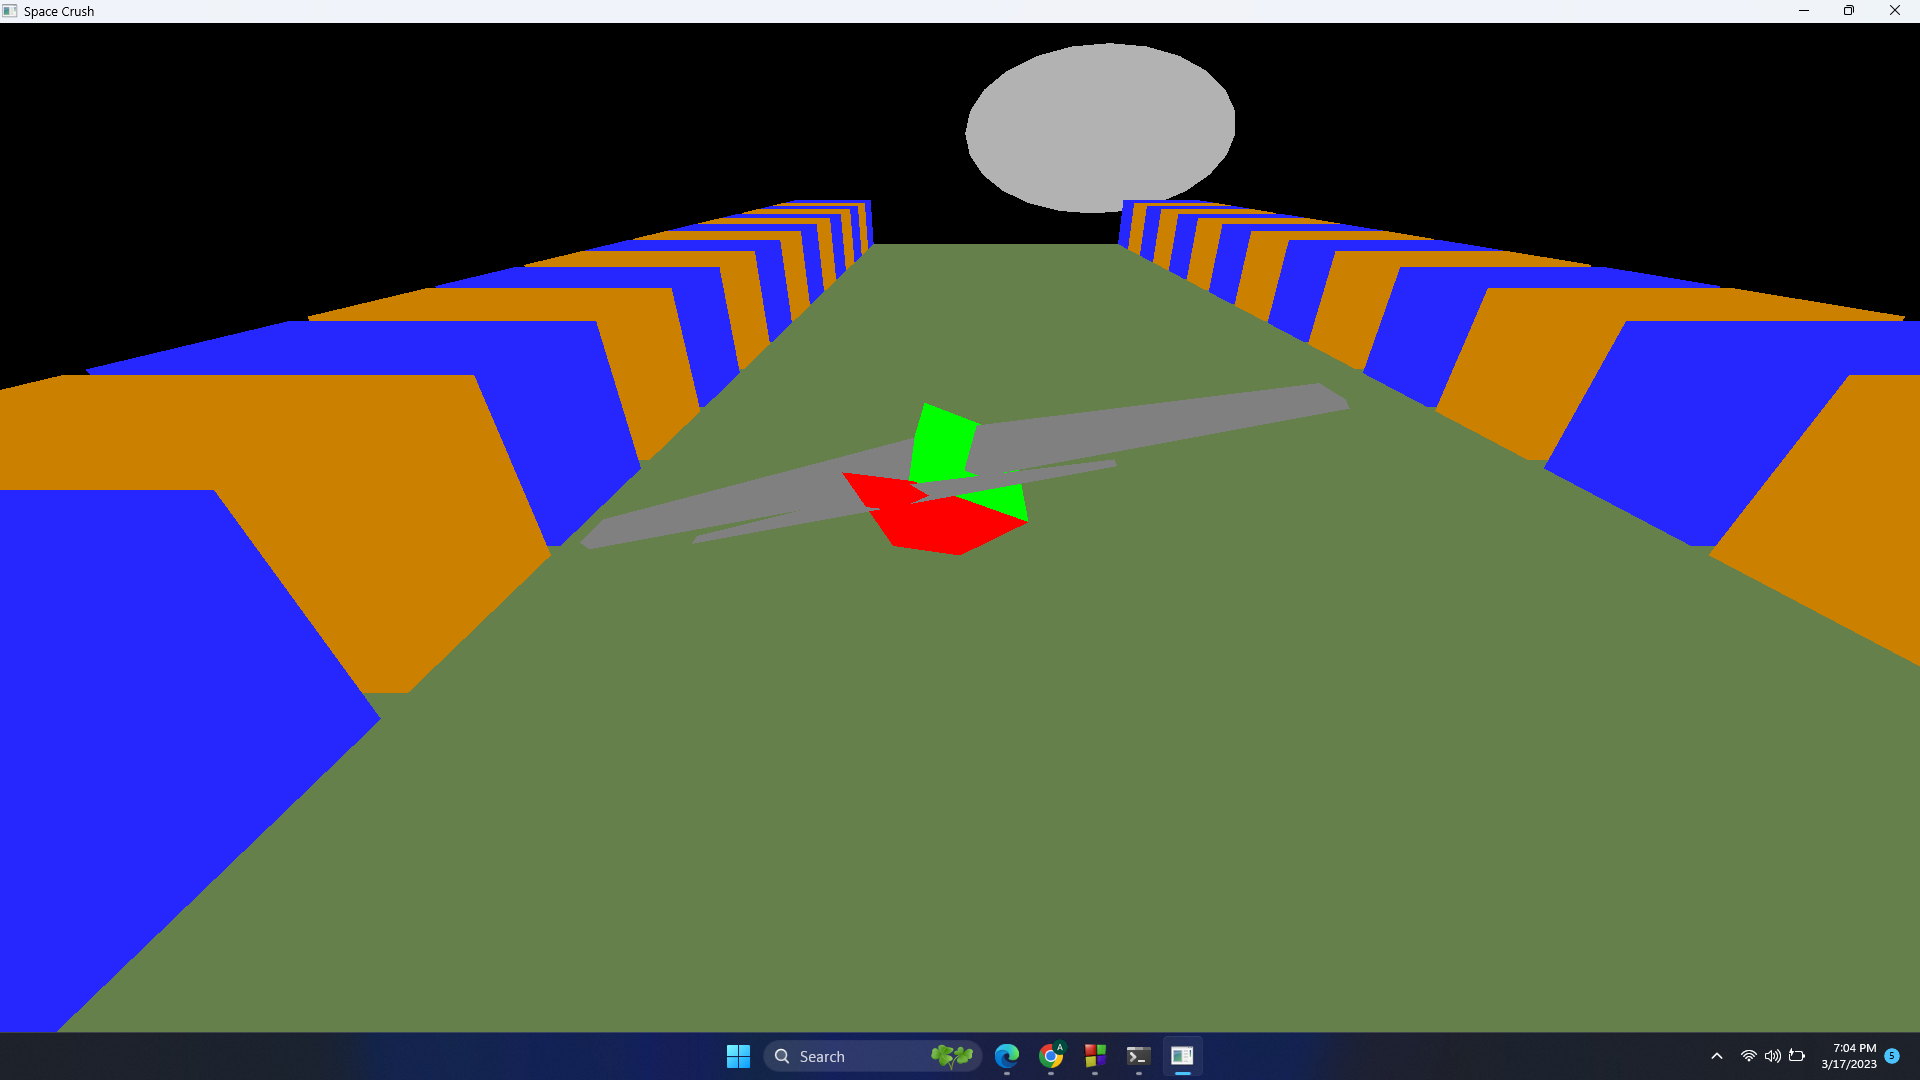
\includegraphics[width=0.7\textwidth, height=7cm]{Screenshot (50).png}
    \caption{Left tilt by pressing 'A' key}
    \label{fig:my_label}
\end{figure}\\

\begin{figure}[h]
    \centering
    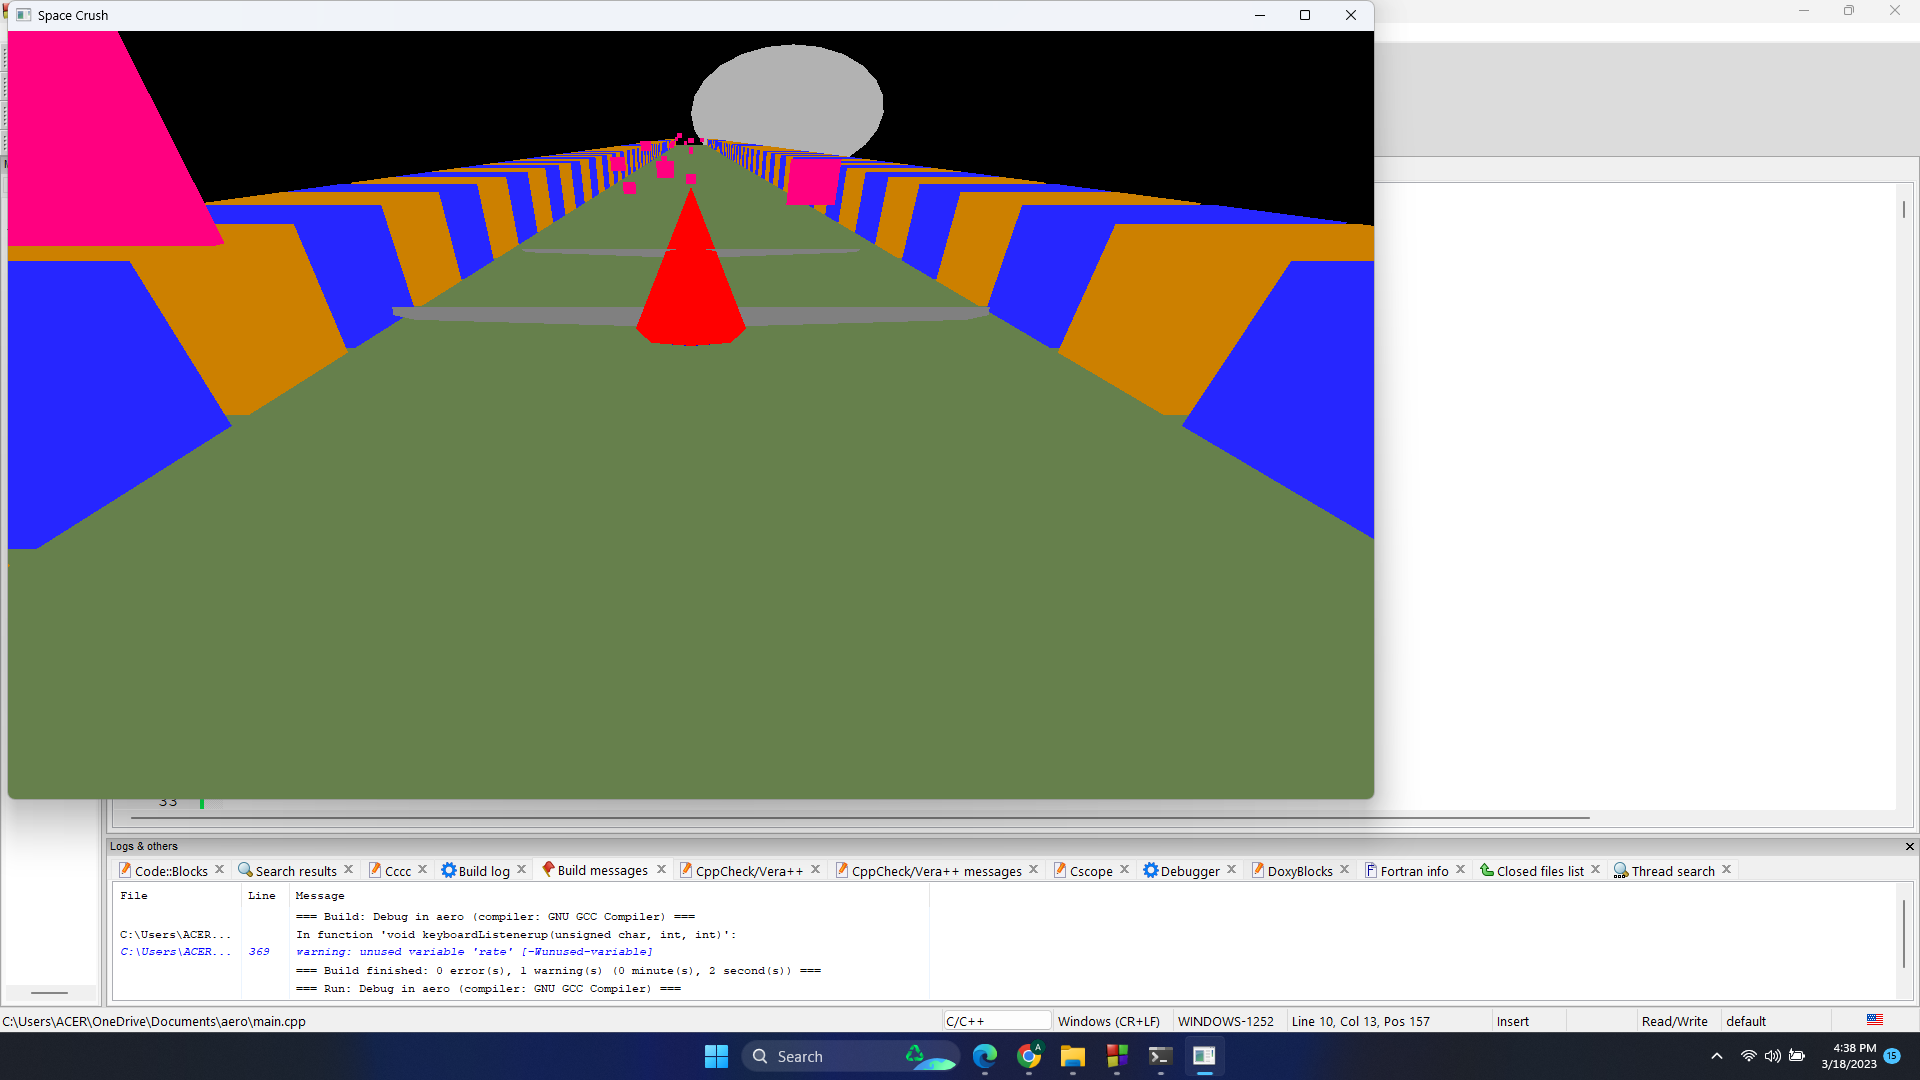
\includegraphics[width=0.7\textwidth, height=7cm]{Screenshot (66).png}
    \caption{Vertical descending by pressing 'W' key}
    \label{fig:my_label}
\end{figure}\\

\begin{figure}[h]
    \centering
    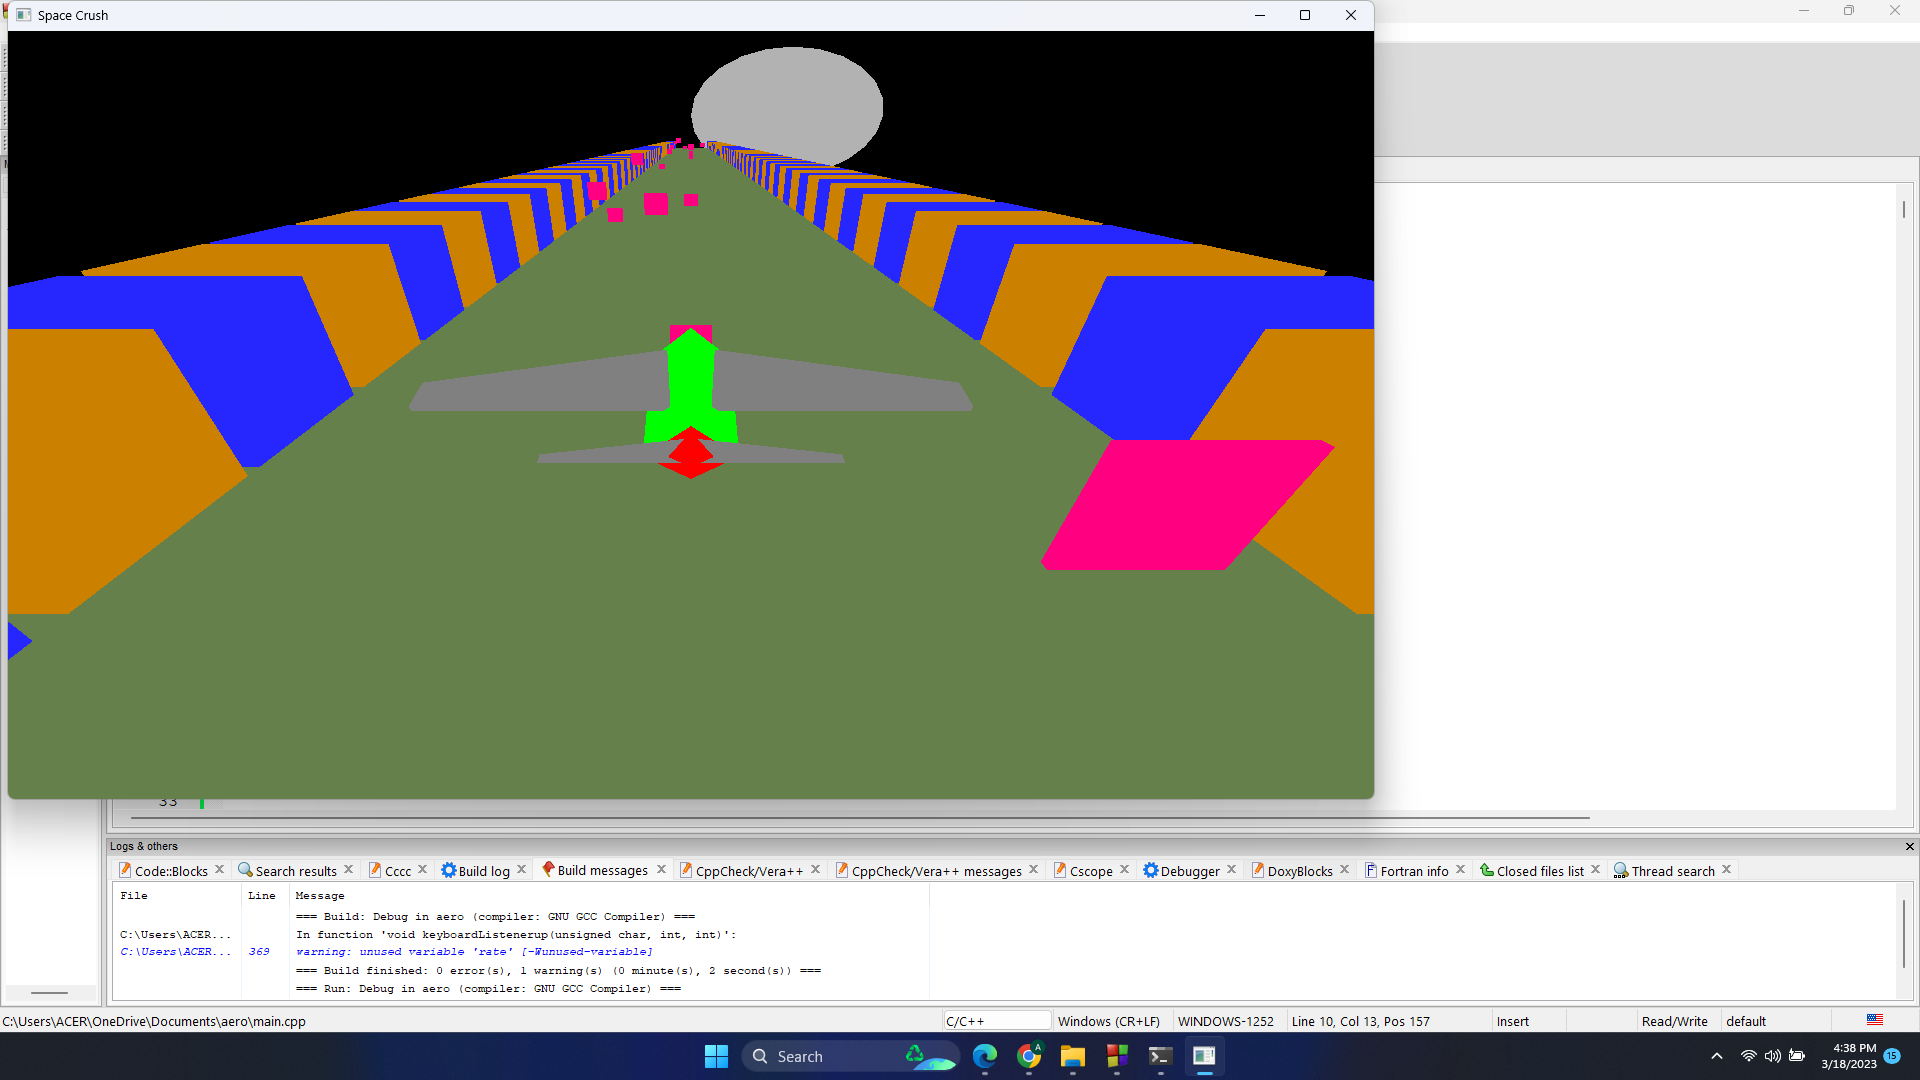
\includegraphics[width=0.5\textwidth, height=7cm]{Screenshot (67).png}
    \caption{Vertical ascending by pressing 'S' key}
    \label{fig:my_label}
\end{figure}\\

\newpage
\textbf{\Large{Mouse control for button and control}}\\
This is a function in C/C++ that listens for mouse events such as button clicks and movements. The function takes four parameters: button, state, x, and y. The button parameter represents the mouse button that was clicked (GLUT\_LEFT\_BUTTON, GLUT\_RIGHT\_BUTTON, or GLUT\_MIDDLE\_BUTTON). The state parameter represents the state of the button (GLUT\_DOWN or GLUT\_UP). The x and y parameters represent the screen coordinates where the event occurred.
In this particular code snippet, the function contains a switch statement that handles different mouse events based on the value of the button parameter. For example, if the left mouse button was clicked and the state is GLUT\_DOWN, the code inside the if statement will be executed.

The commented out code inside the if statement appears to be calculating the X and Z coordinates of a bullet based on the current angle of the camera and turret.

Similarly, if the right mouse button was clicked and the state is GLUT\_DOWN, the value of the drawaxes variable is toggled between 0 and 1.

If the default case is reached (i.e. none of the other cases matched), the code appears to adjust the angle of the camera and turret based on the direction of the mouse movement.
\section{\Huge{User Guide}}
\subsection{\Large{Build Instruction}}
Building the project requires:\\
\begin{itemize}
    \item codeblock compiler at \url{https://www.codeblocks.org/downloads/}\\
    \item Glut \url{http://www.xmission.com/~nate/glut.html}\\
    \item for further tutorial to set up glut in codeblocks check at: \url{https://www.youtube.com/watch?v=uOlV4x28KgI}\\
    \end{itemize} 
    \begin{figure}
        \centering
        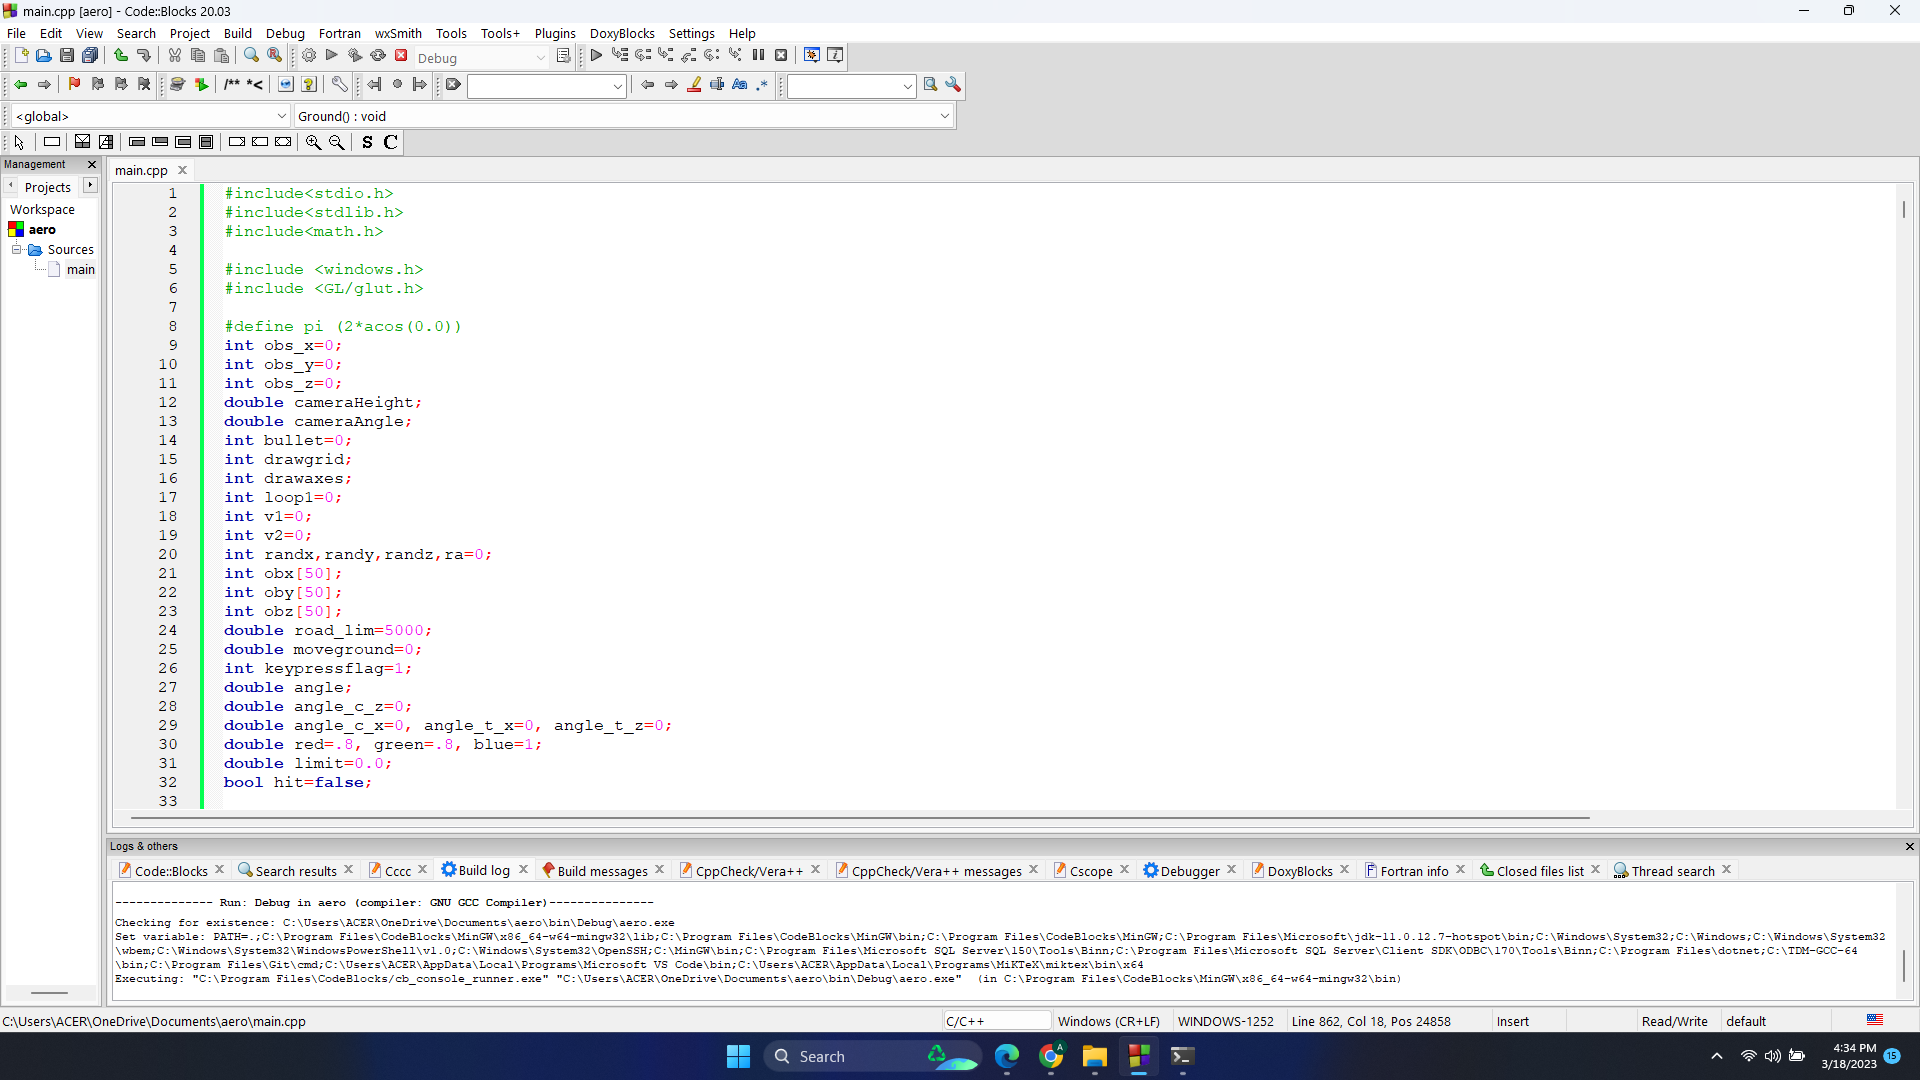
\includegraphics[width=0.75\textwidth, height=7cm]{Screenshot (63).png}
        \caption{A cross platform as Code Blocks}
        \label{fig:my_label}
    \end{figure}

    \newpage
\subsection{\Large{Game Guide}}
\begin{table}[h]
    \centering
    \begin{tabular}{|c||c|}
    \hline
       & \textbf{\large{key}} & \textbf{\large{fuction}} \\ \hline
       & forward arrow & to move camera forward \\ \hline
       & backward arrow & to move camera backward \\ \hline
       & Q & to make face of Airplane face at some angle in left side \\ \hline
       & W & to make descending in altitude of flying object \\ \hline
       & E & to make face of Airplane face at some angle in right side \\ \hline
       & A & to make Airplane tilt in left side \\ \hline
       & S & to make ascending in altitude of flying object \\ \hline
       & D & to make airplane tilt in right side \\ \hline
    \end{tabular}
    \caption{A table for control keys for operation of game}
\end{table}\\

\newpage
\section{\Huge{Discussion}}
Even at this stage the sky is the limit to where to take the project further, the architecture
supports expansion in any way possible.

All members enhanced and reinforced concepts learnt in class and increased their capacity to
take on challenging Graphics related projects additionally lessons were learned in management
and software processes essential to deliver quality code on time.

We have no regrets over the decision we made in regards to development of individual
components. If more time given more functionality would be present. Use of libraries
worked in both ways for us, codeblocks allowed us to add cross platform features and sound though it
also didn’t allow us to port the GUI component in game on time. Incidents like this are natural
and not unexpected.

In future work aspects listed in unimplemented features could be completed additionally since
all components were built individually it would be worth to begin utilizing more robust external
libraries in areas of physics and graphics engine.
\section{\Huge{Conclusion}}
The project on the whole presented a challenge, the course is different from other programming
courses offered since there is a subjective parameter that’s hard to measure. The team took on
many challenges to bring the deliverable to this stage and all are pleased with the effort and the
end result.
\end{document}
